\chapter{Launch and Astrodynamic Characteristics}
\label{frLaAC}
This chapter explains the characteristics of the launch and space segments of the mission. Section \ref{frLS} describes the three main characteristics of bringing the swarm into the orbit: launch vehicle, launch location and orbit insertion. Section \ref{frSS} discusses all the aspects of the constellation and its configuration, and delves into estimations of $\Delta$V and needed propellant. Finally, section \ref{frSEaS} deals with the hazardous space environment and ways of protecting the satellites against it. 

\section{Launch Segment}
\label{frLS}

The launch segment of the mission includes the selection of the launch vehicle, the launch location and the procedure of inserting the satellites into their respective orbits. The following subsections discuss all of these aspects. 

\subsection{Launch Vehicle}
\label{frLSLV}

HERE ADD VIBRATION ANALYSIS

\subsubsection{Cost and Reliability Analysis}
\label{frLVCA}

The costs of launch vary greatly between different vehicles. Table \ref{table:vehicleCosts} on page \pageref{table:vehicleCosts} lists approximate total launch costs of respective platforms. The prices are given in Fiscal Year 2000 dollars for consistency.
\begin{table}[h]
\begin{centering}
\begin{tabular}{llr}
\toprule
Platform & Operator & Price (FY00\$m) \\
\midrule
Ariane V  & ESA & 97.96 \\
Soyuz   & Starsem    &  8.16 - 22.1 \\
Vega   & European and Italian SA  & 15.1 \\
Falcon 1E  & SPACEX  & 8.89 \\
PSLV & ISRO & 13.88 - 16.33 \\
Rokot & Eurokot & 9.8 - 11.4 \\
\bottomrule
\end{tabular}
\caption{Estimated price comparison of different launch vehicles. \emph{Source: various.}}
\label{table:vehicleCosts}
\end{centering}
\end{table}

Based on the information  in the above table it is possible to single out a few platforms which will be affordable for the purpose of this feasibility study. The Ariane V launcher is the most expensive option by far and would push the budget quite heavily, with an estimated cost of launch almost half of the total budget. However the payload capabilities of the Ariane V launcher far outweigh that of all other platforms, thus making it possible for a combined launch with other satellites, leading to shared costs. This however could jeopardize the mission in the sense that it becomes secondary priority. If that happens, the constellation would have have have higher requirements for orbit acquisition: an extra booster stage or higher onboard fuel capacity for the altitude and/or plane shift, which is not feasible. The Ariane V is therefore an unsuitable platform for this project. 

The rest of the launchers can be analyzed with respect to reliability. All of the launch vehicles have been tested, with the exception of the Vega system, which is yet to make its maiden flight. The Vega is therefore not suitable for the analysis at this time. It is for this reason that the project will no longer consider this system at all.  However, better data should be available in the near future which should allow for the Vega platform to be reevaluated.

The same goes for the Falcon - 1e system. The launcher is still under development. Furthermore, the predecessor of the 1e system is the Falcon - 1, which out of total of five launches only had two successful, fails to make a favorable impression. 

Table \ref{table:LVreliability} on page \pageref{table:LVreliability} shows some reliability statistics for the remaining 3 vehicles.

\begin{table}[h]
\begin{centering}
\begin{tabular}{lcccp{5cm}}
\toprule
Platform & Total No. of Launches & Total Failures & Reliability & No. of Successful Launches Since Last Failure  \\
\midrule
Soyuz   & 1754  &  88 & 95\% & 57 \\
PSLV & 16 & 1 & 94\% & 15 \\
Rokot & 17& 2 & 88\% & 6 \\
\bottomrule
\end{tabular}
\caption{Reliability figures for several launch vehicles. \emph{Source: various.} }
\label{table:LVreliability}
\end{centering}
\end{table}

The Soyuz launch vehicle presents itself as the most reliable platform, with a track record that far surpassed all other options. This launch vehicle will be the one considered for this project. In the next section, its payload capabilities are discussed.

\subsubsection{Soyuz LV Payload Capability Analysis}
\label{frLVPCA}

There is a large selection of Soyuz vehicles available for consideration. For the purpose of this project, the newest modification - Soyuz-ST will be used. This vehicle is part of the Soyuz-2 family, which are technologically superior to the older Soyuz-U and U2 launchers. An illustration and technical parameters of the Soyuz-ST can be found in Appendix \ref{appa} on page \pageref{appa} \cite{soyuzman}.

An estimation of mass performance for the launch vehicle can be seen in figure \ref{fig:massperformance} on page \pageref{fig:massperformance}.

\begin{figure}[ht]
\centering
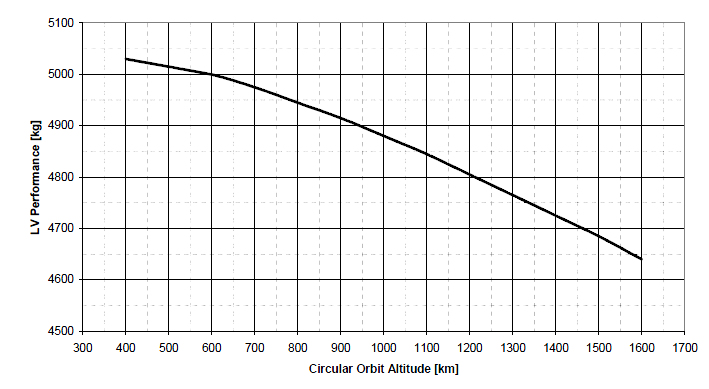
\includegraphics[width=1.0\textwidth, angle=0]{chapters/img/lvmass.png}
\caption{Mass performance of the Soyuz-ST for circular Orbits.\emph{ Source: \cite{soyuzman}.}}
\label{fig:massperformance}
\end{figure}

The payload mass data provided in \cite{soyuzman} is estimated, yet is good enough to have a reasonable idea about the maximum mass. The Soyuz-ST is able to launch roughly a maximum of 5000 kg into a 500km orbit. This is well above the design mass of the formation thus will allow for further considerations of joint launches (as long as the swarm mission is considered to be the primary payload) and thus spread launch costs. 

The available volume in the Soyuz-ST Fairing can be seen in figure \ref{fig:soyuzvol} on page \pageref{fig:soyuzvol}.

\begin{figure}[!h]
\centering
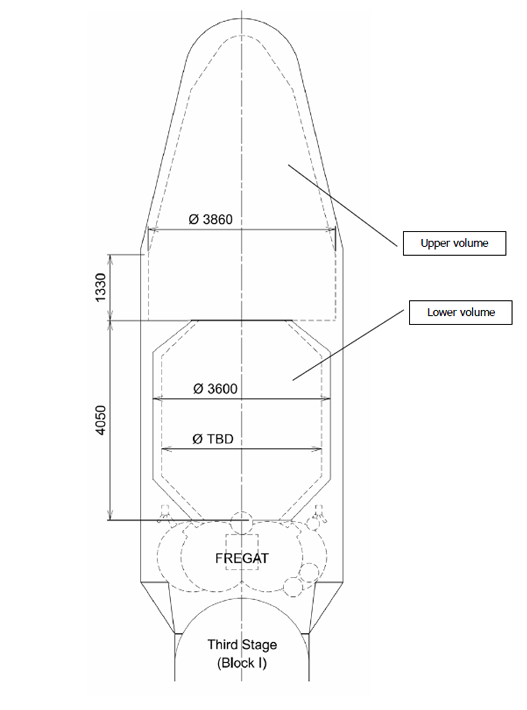
\includegraphics[scale = 0.5, angle=0]{chapters/img/soyuzvol.png}
\caption{Fairing volume of the Soyuz-ST launch vehicle.\emph{ Source: \cite{soyuzman}.}}
\label{fig:soyuzvol}
\end{figure} 

The dimensions of the fairing are visibly too large and there is no possibility of using a different one, however that leaves a lot of possibilities for different designs of release adapters to adapt to the unique sequence of separation upon orbit injection. Again, the possibility of taking other small satellites along on the same launch arises.  

\subsection{Launch Site}
\label{frLSLS}

The selection of the launch site relies on several factors:

\begin{itemize}
	\item Availability of attainable inclinations from launch.
	\item Compatibility with the launch vehicle.
	\item Accessibility and cost.
	\item Security and political reasons. 
\end{itemize}

The first factor is crucial. It is paramount that the satellites are injected into their final inclinations at launch and do not have to perform any inclination change maneuvers, which require a substantial $\Delta$V. With this in mind choosing a launch site closer to the equator is necessary. Launch sites at higher latitudes would need to sacrifice velocity and thus payload mass because of their location. Table \ref{table:launchtable} on page \pageref{table:launchtable} shows a number of possible launch sites and their locations \cite{larson}. The list contains only the sites compatible with the Soyuz-ST launch vehicle. Furthermore, in figure \ref{fig:launchsites} on page \pageref{fig:launchsites}, the same sites are indicated with their respective authorized inclination ranges.

\begin{table}[!h]
\begin{centering}
\begin{tabular}{llp{2cm}p{2cm}}
\toprule
Launch Site & Operator & Latitude (deg min) & Longitude (deg min) \\
\midrule
Baikonur LC-31/6  & Russia (Starsem) & 45 54 N & 63 18 E \\
Plesetsk LC-43  & Russia (Starsem)   &  62 48 N & 40 24 E \\
Guiana Space Centre  ELS  & CNES/Arianespace  & 5 18 N & 52 50 W \\
\bottomrule
\end{tabular}
\caption{Available launch sites for the Soyuz-ST.   \emph{Source: \cite{larson}.}}
\label{table:launchtable}
\end{centering}
\end{table}  

\begin{figure}[!h]
\centering
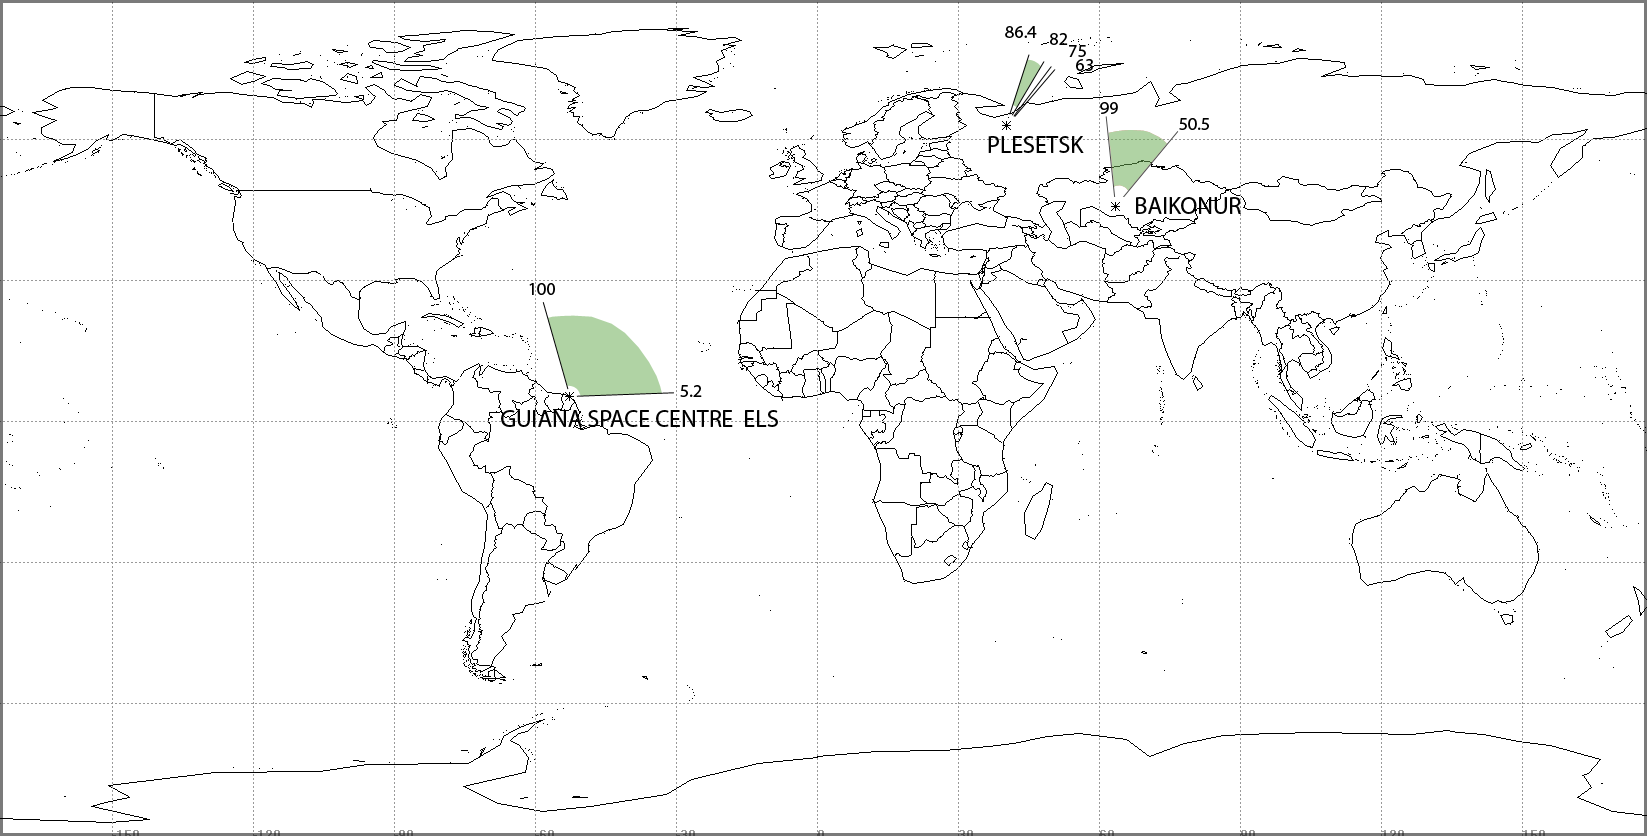
\includegraphics[width=1.0\textwidth, angle=0]{chapters/img/launchsites.png}
\caption{Launch site locations and allowable inclinations for the Soyuz-ST.}
\label{fig:launchsites}
\end{figure}

\subsection{Orbit Acquisition}
\label{frLSOI}

Once the final stage of the launch vehicle has reached desired orbit altitude and inclination, preparations can start for proper separation maneuvers. This maneuver has to be designed in such a way as to accommodate all phase shifts required by the satellite orbits. Using the 

\section{Space Segment}
\label{frSS}

\subsection{Emitter Orbit}
\label{frSSEOD}

bla

\subsection{Receiver Orbits}
\label{frSSRO}

b lss

\subsection{Collision Avoidance}
\label{frSSCA}

bla

\subsection{Stationkeeping}
\label{frSSS}

bla

\section{Space Environment and Shielding}
\label{frSEaS}

Bla